\refstepcounter{chapter}
\addcontentsline{toc}{chapter}{Work Tables}

\section{Fixed Angle Table}

\subsection*{Application}
The fixed angle table has a rectangular shape and is used to hold bulky workpieces during machining operations that do not require an angular adjustment of the workpiece.

The fixed angle table is fastened to the machine’s vertical clamping table using T-slot nuts and hex bolts.

\subsection*{Technical Data}

\begin{itemize}
   \item \textbf{Clamping surface} \dotfill 800 x 250mm
   \item \textbf{Number of T-slots (14 H7)} \dotfill 4
   \item \textbf{Distance between T-slots} \dotfill 63mm
   \item \textbf{Weight (approx.)} \dotfill 100kg
   \item \textbf{Maximum table load (incl. workpiece and clamping tools)} \dotfill 200kg
\end{itemize}


\sectionLikeSubsection{Fixed Angle Table - Working Area Dimensions}

\vspace{3cm}

\begin{center}
    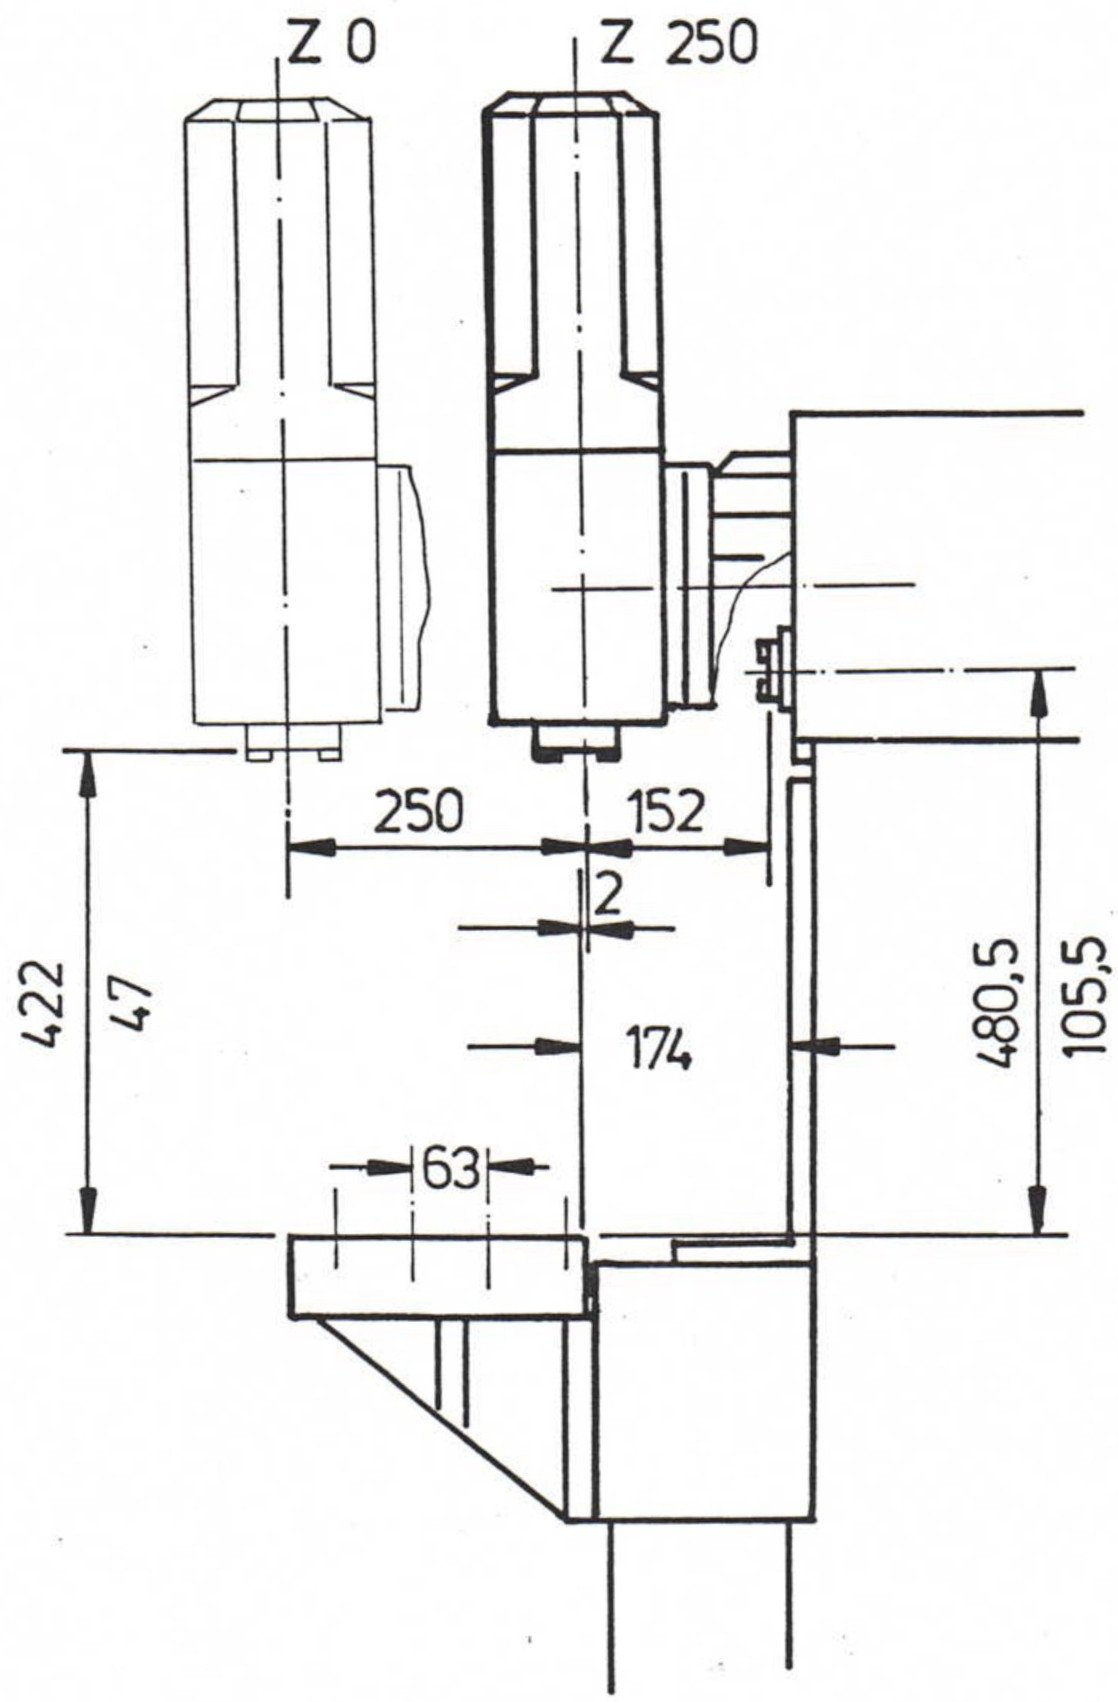
\includegraphics[width=.7\textwidth]{chapter4/fixed_angle_table_dimensions.jpg}    
\end{center}

\section{Universal Built-in Rotary Table with ROD Encoder}

\setcounter{section}{3}

\subsection*{Application}

The universal built-in rotary table is used for holding heavy and large workpieces during complex spatial machining operations that require high geometric precision.

To adjust the spatial angle, the table can tilt around both its transverse and longitudinal axes by ±30°, and the table plate can rotate 360°.

The table is equipped for indirect dividing.

The table plate is manually clamped.

\subsection*{Technical Data}

\begin{itemize}
   \item \textbf{Clamping surface} \dotfill 550 x 280mm
   \item \textbf{Centering bore} \dotfill 30 H7mm
   \item \textbf{Number of T-slots (14 H7)} \dotfill 4
   \item \textbf{Distance between T-slots} \dotfill 63mm
   \item \textbf{Tilting range around transverse axis} \dotfill ±30°
   \item \textbf{Tilting range around longitudinal axis} \dotfill ±30°
   \item \textbf{Rotational range of table plate} \dotfill 360°
   \item \textbf{Encoder with digital display, resolution} \dotfill 0.001°\footnotemark
   \item \textbf{Indirect dividing using handwheel:}
   \begin{itemize}
       \item Overall gear ratio \dotfill 90:1
       \item One full turn of handwheel \dotfill 4°
       \item One scale division on table \dotfill 20'
   \end{itemize}
   \item \textbf{Maximum table load (incl. workpiece and clamping tools)} \dotfill 150kg
   \item \textbf{Weight (approx.)} \dotfill 75kg
\end{itemize}

\footnotetext{Not included in versions without ROD.}

\sectionLikeSubsection{Universal Built-in Rotary Table}

\begin{figure}[h]
    \centering
    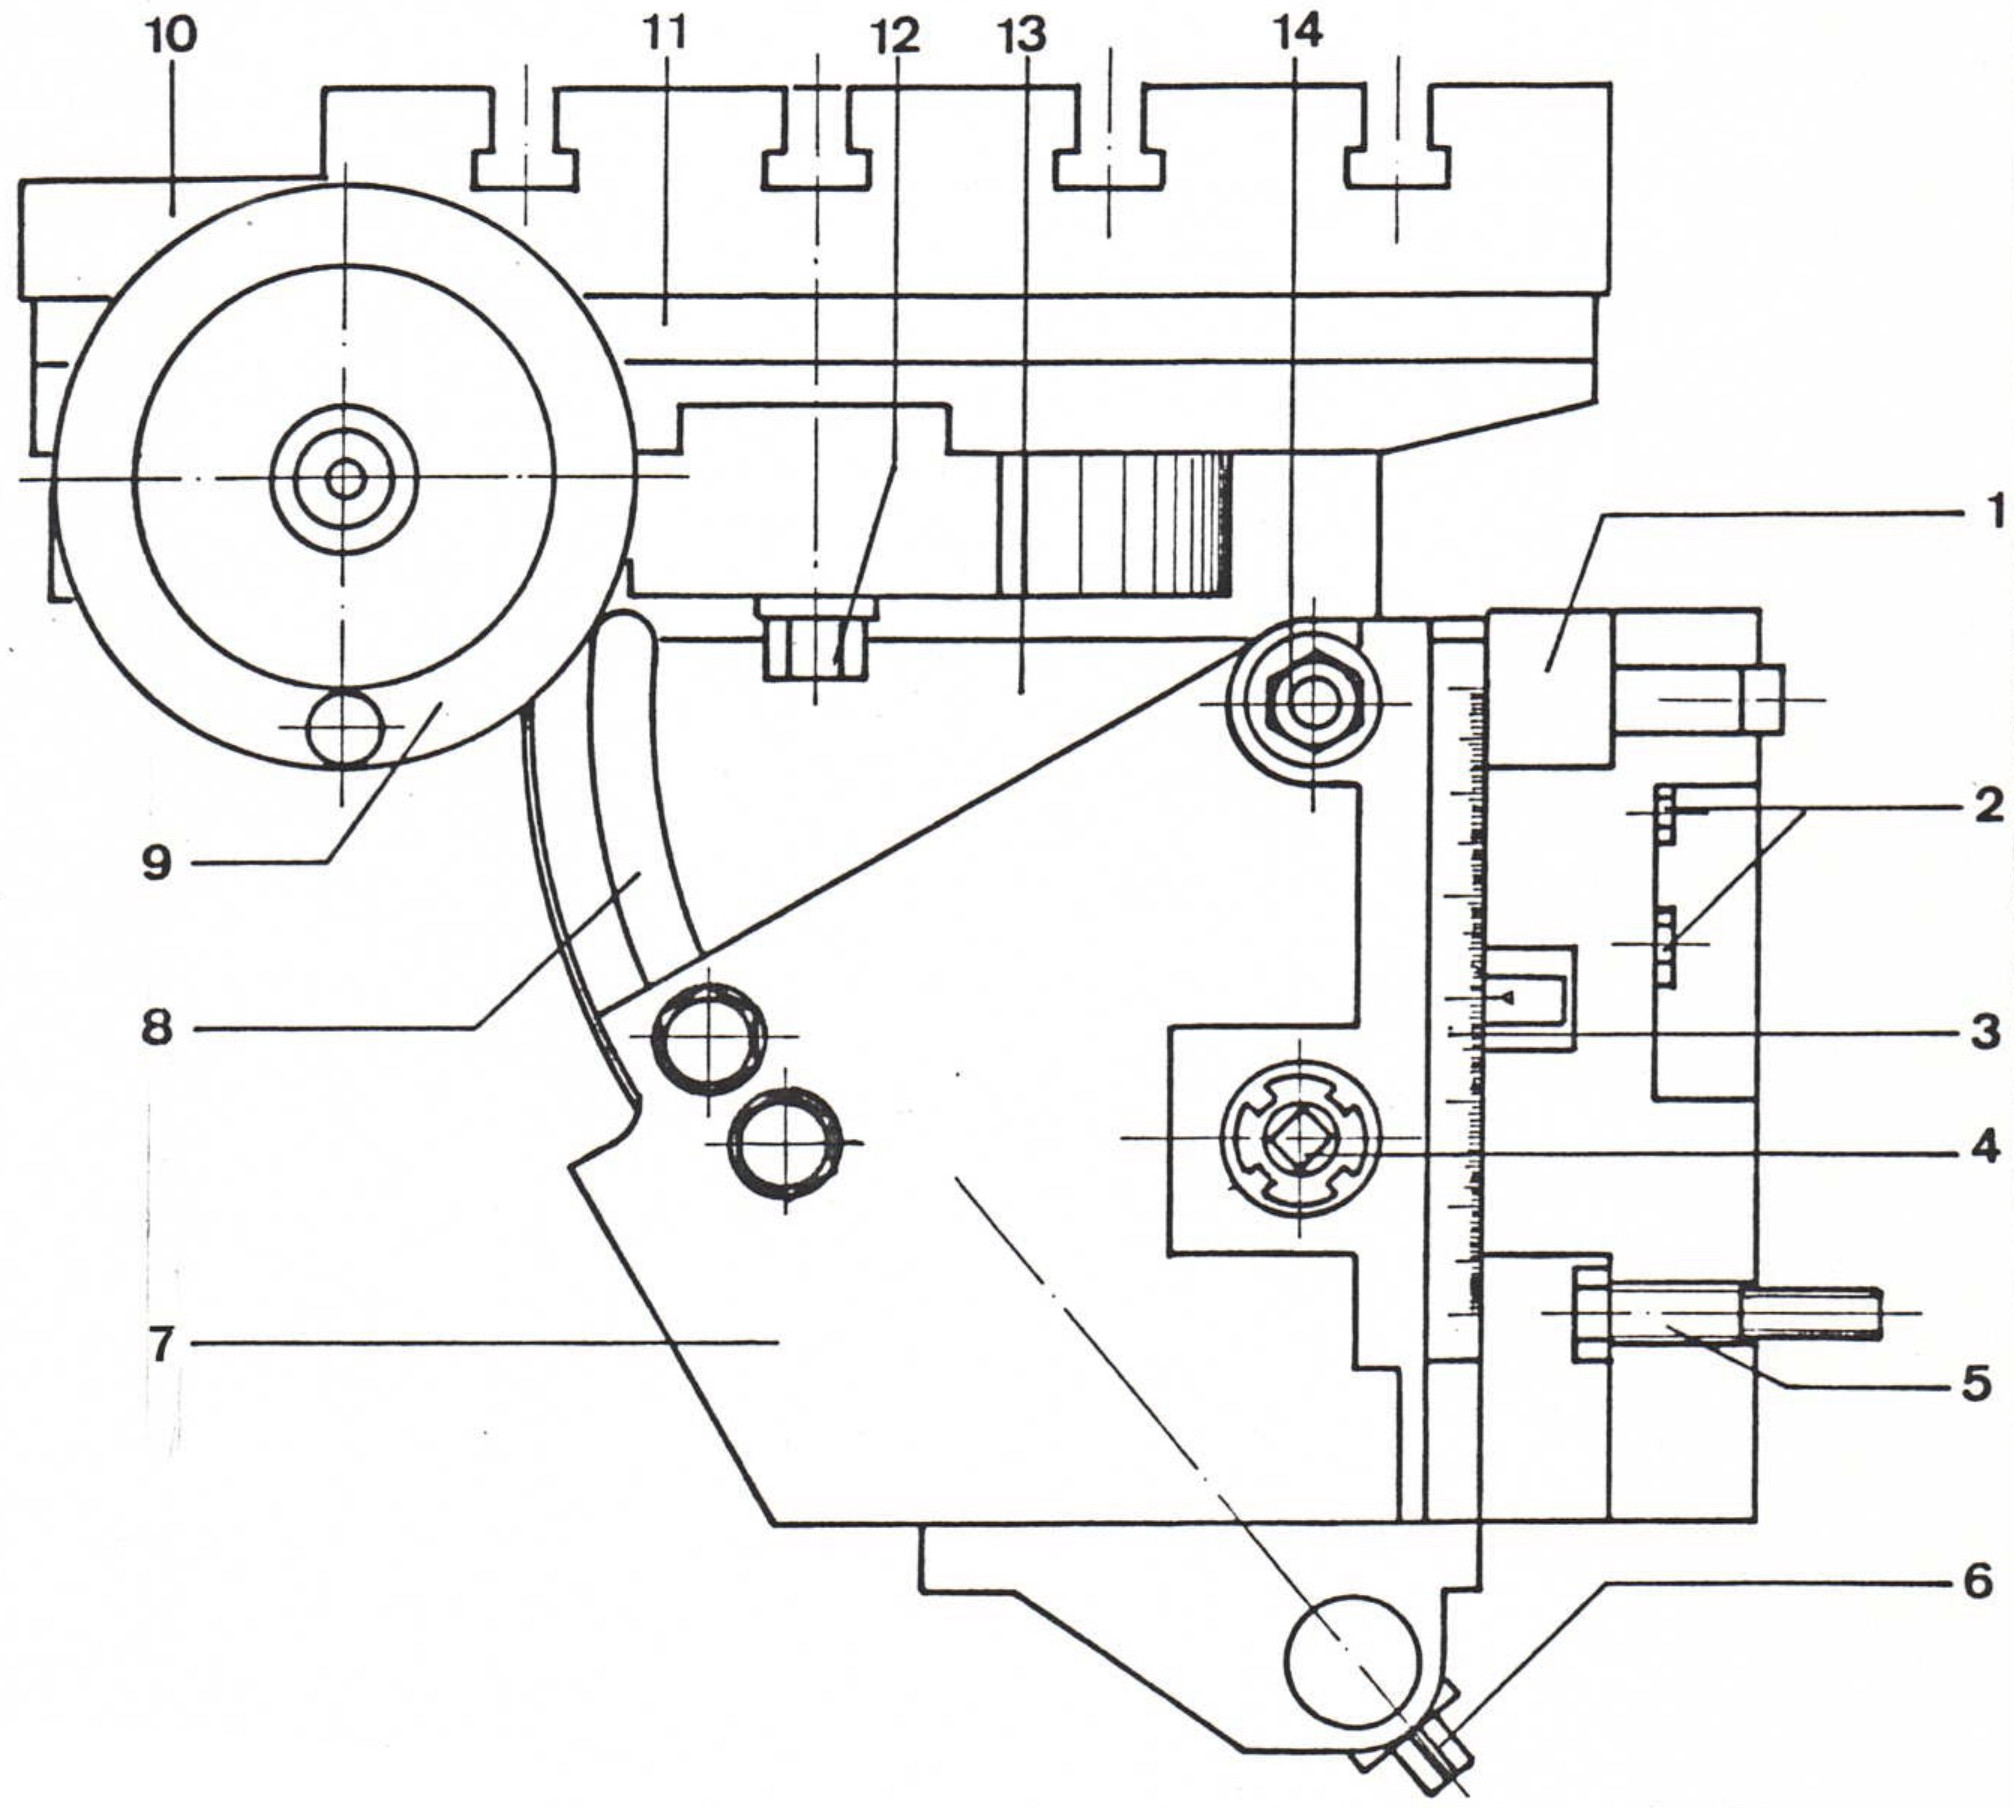
\includegraphics[width=0.8\textwidth]{chapter4/universal_rotary_table.jpg}
\end{figure}

\begin{enumerate}
    \item \textbf{Clamping plate}
    \item \textbf{Clamping screws for securing the console to the clamping plate}
    \item \textbf{Scale for reading the swivel angle of the console} (1 division = 20')
    \item \textbf{Square drive for swiveling the console around the transverse axis}
    \item \textbf{Hex bolts and T-slot nuts for securing the clamping plate} to the machine's vertical clamping table
    \item \textbf{Square drive for swiveling the swivel section around the longitudinal axis}
    \item \textbf{Console}
    \item \textbf{Scale for reading the swivel angle of the swivel section} (1 division = 10')
    \item \textbf{Handwheel drive for indirect dividing according to the table scale} (1 full turn = 4°)
    \item \textbf{Table plate, rotatable by 360°}
    \item \textbf{Scale for reading the rotation angle of the table plate} (1 division = 20')
    \item \textbf{Nuts for securing the table plate to the swivel section}
    \item \textbf{Swivel section}
    \item \textbf{Clamping screws for securing the swivel section in the console}
\end{enumerate}

\sectionLikeSubsection{Operating the Universal Built-in Rotary Table}

\begin{figure}[h]
    \centering
    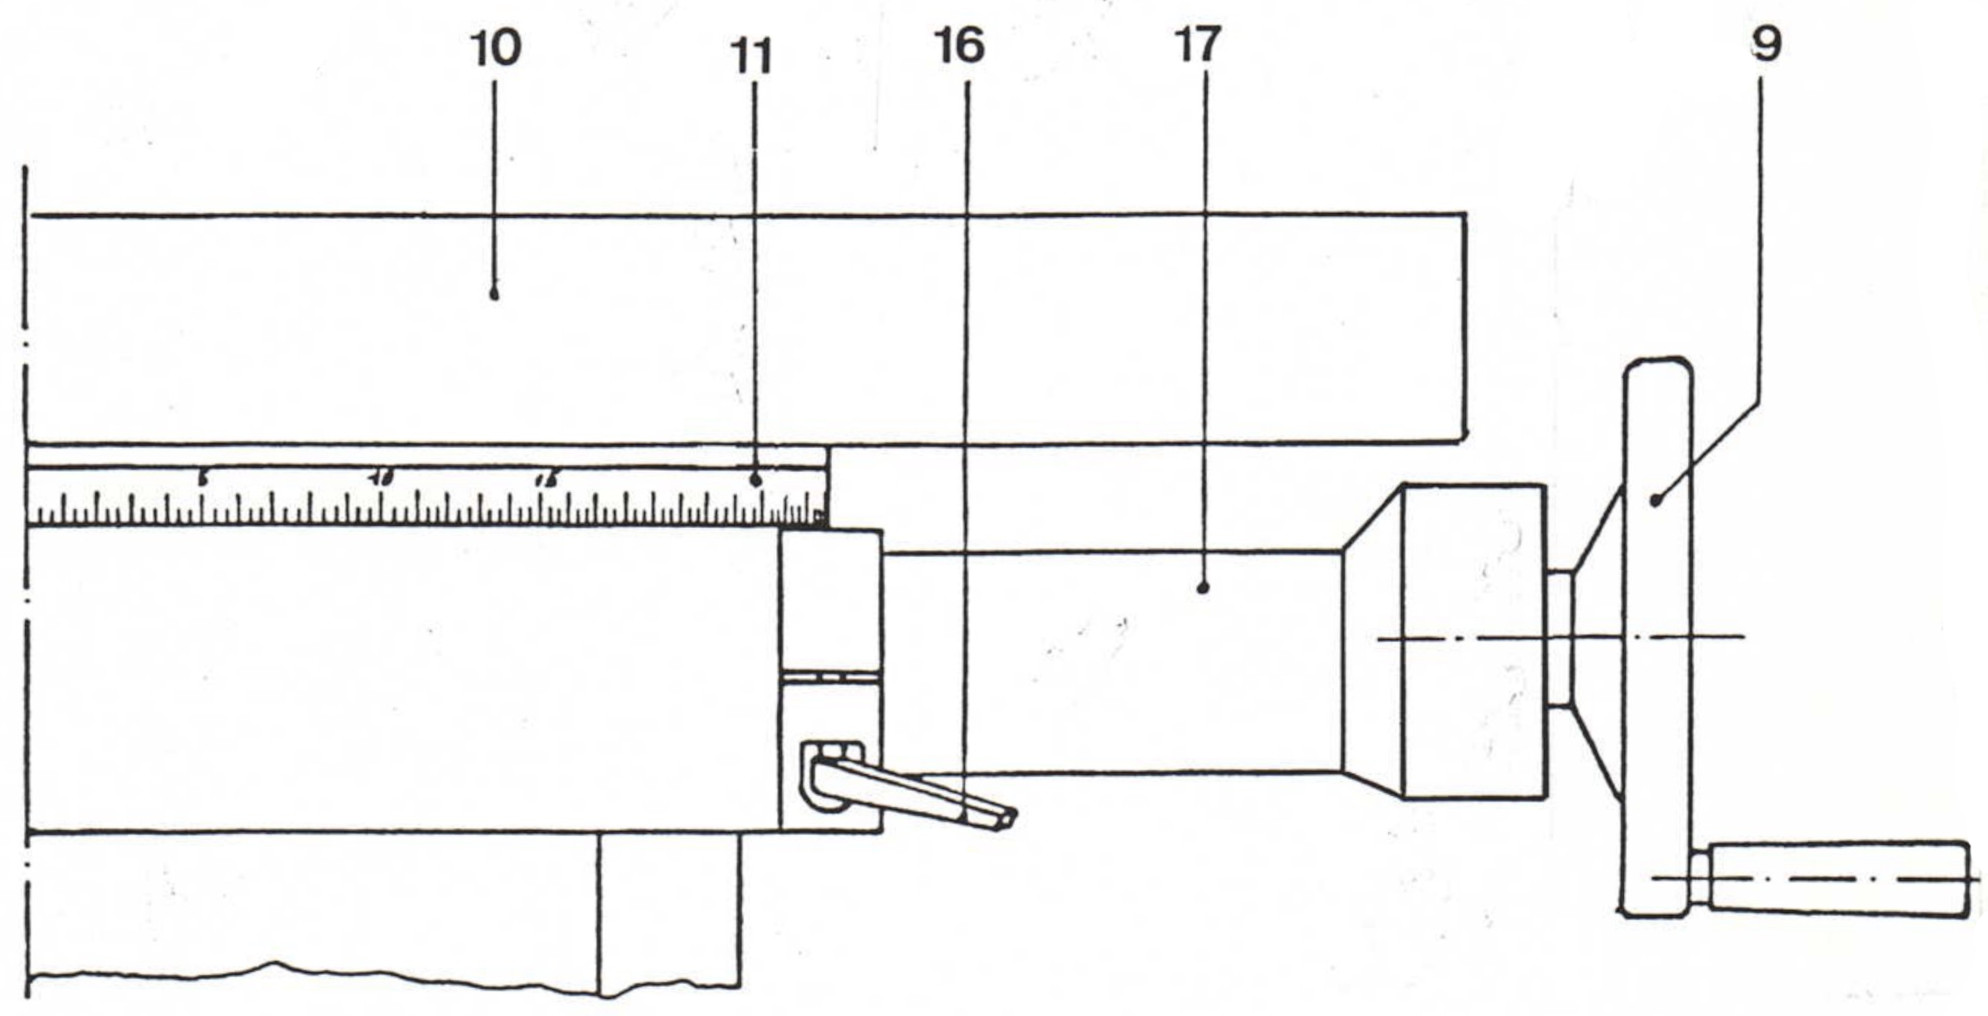
\includegraphics[width=0.8\textwidth]{chapter4/universal_rotary_table_operation.jpg}
\end{figure}

\begin{enumerate}
    \item[16] \textbf{Clamping lever for securing the eccentric bushing} of the indexing worm.
    \item[17] \textbf{Eccentric bushing for engaging the indexing worm externally} for indirect dividing.
\end{enumerate}

\subsection*{Working with the Universal Built-in Rotary Table}
\begin{itemize}
    \item Before swiveling the table around its horizontal transverse axis, all clamping screws (2) must be loosened.
    \item Before swiveling the table around its horizontal longitudinal axis, all clamping screws (14) on both sides of the console must be loosened.
    \item When performing indirect dividing, the handwheel (9) must always be rotated in the same direction to eliminate any influence of backlash in the dividing gearbox on the indexing accuracy.
    \item The machine spindle must be stopped before each indexing operation.
    \item After each indexing operation, the table plate (10) must be secured again by tightening the nuts (12).
\end{itemize}

\newpage
\subsection*{Indirect Dividing Using Scale Ring}

\begin{itemize}
    \item Loosen the \textbf{nuts (12)} securing the table plate (10).
    \item Loosen the \textbf{clamping lever (16)} and rotate the \textbf{eccentric bushing (17)} to the right until the indexing worm is engaged, then retighten the clamping lever (16).
    \item Rotate the \textbf{handwheel (9)} to set the required rotation angle of the \textbf{table plate (10)} according to the \textbf{scale (11)}.
    \item Retighten the \textbf{nuts (12)}.
\end{itemize}

\notebox{NOTE}{Adjustment operations for the universal built-in rotary table are described in Section 7 of the operator’s manual.}

\subsection*{Lubrication / Maintenance}
\begin{itemize}
    \item Every 200 operating hours, lubricate the three grease nipples with slideway oil \textbf{"GULP 68"}.
\end{itemize}

\begin{figure}[h]
    \centering
    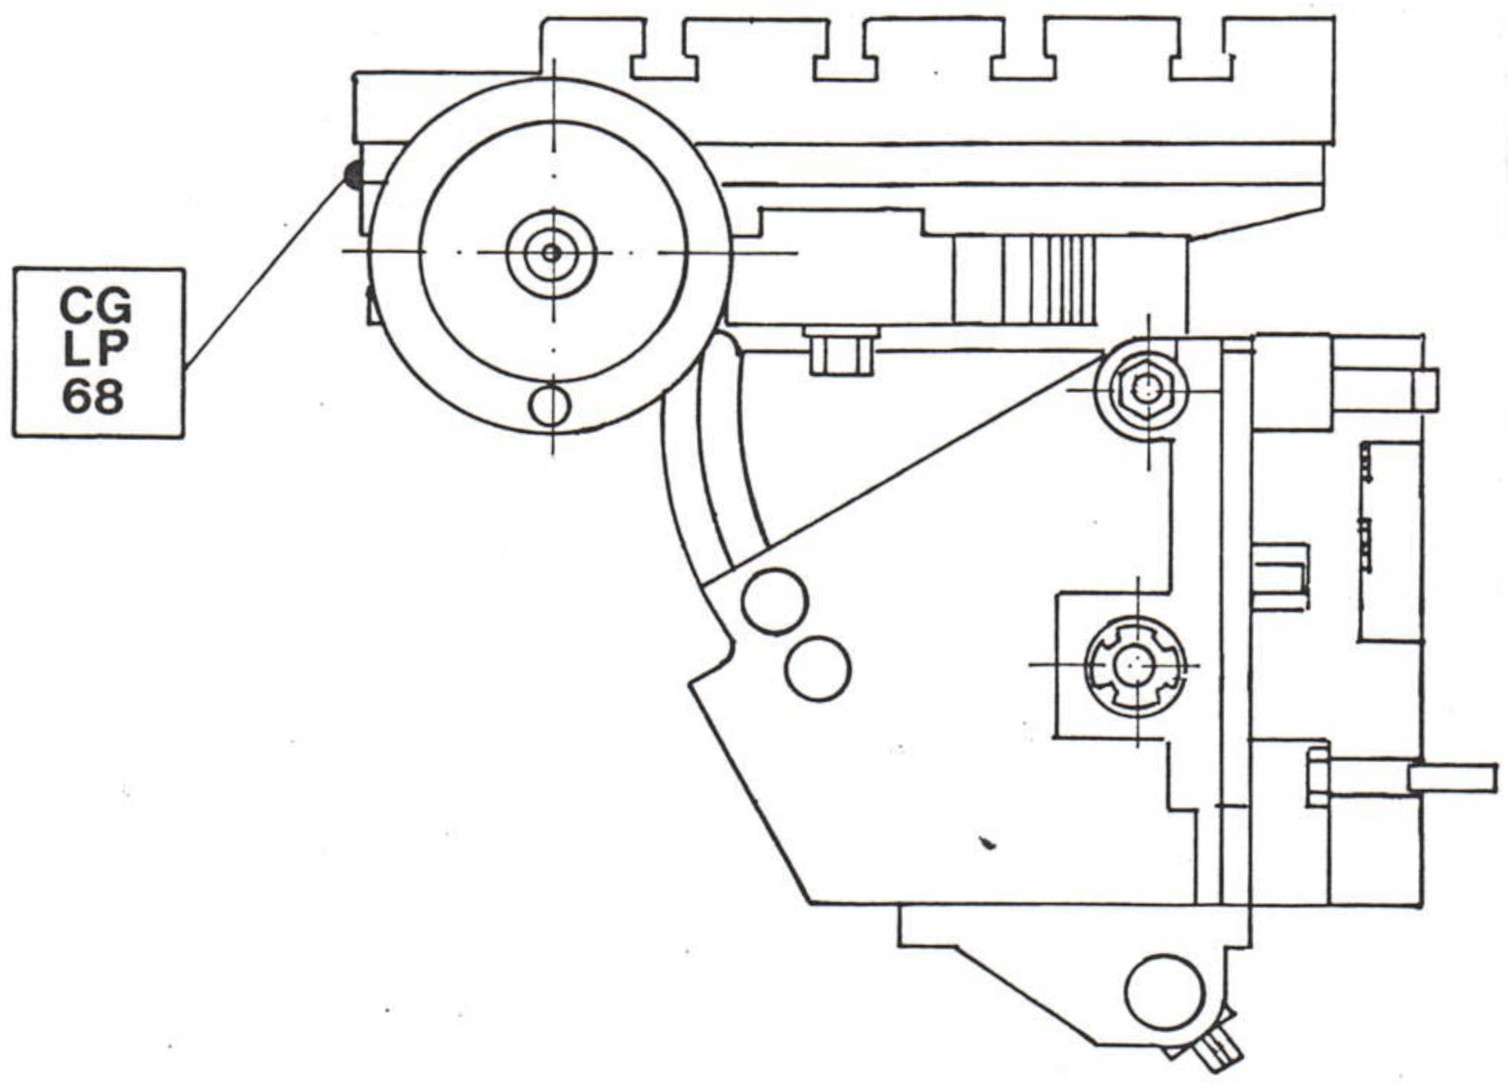
\includegraphics[width=0.8\textwidth]{chapter4/universal_rotary_table_lubrication.jpg}
\end{figure}

\sectionLikeSubsection{Universal Rotary Table - Work Area Dimensions}

\begin{figure}[h]
    \centering
    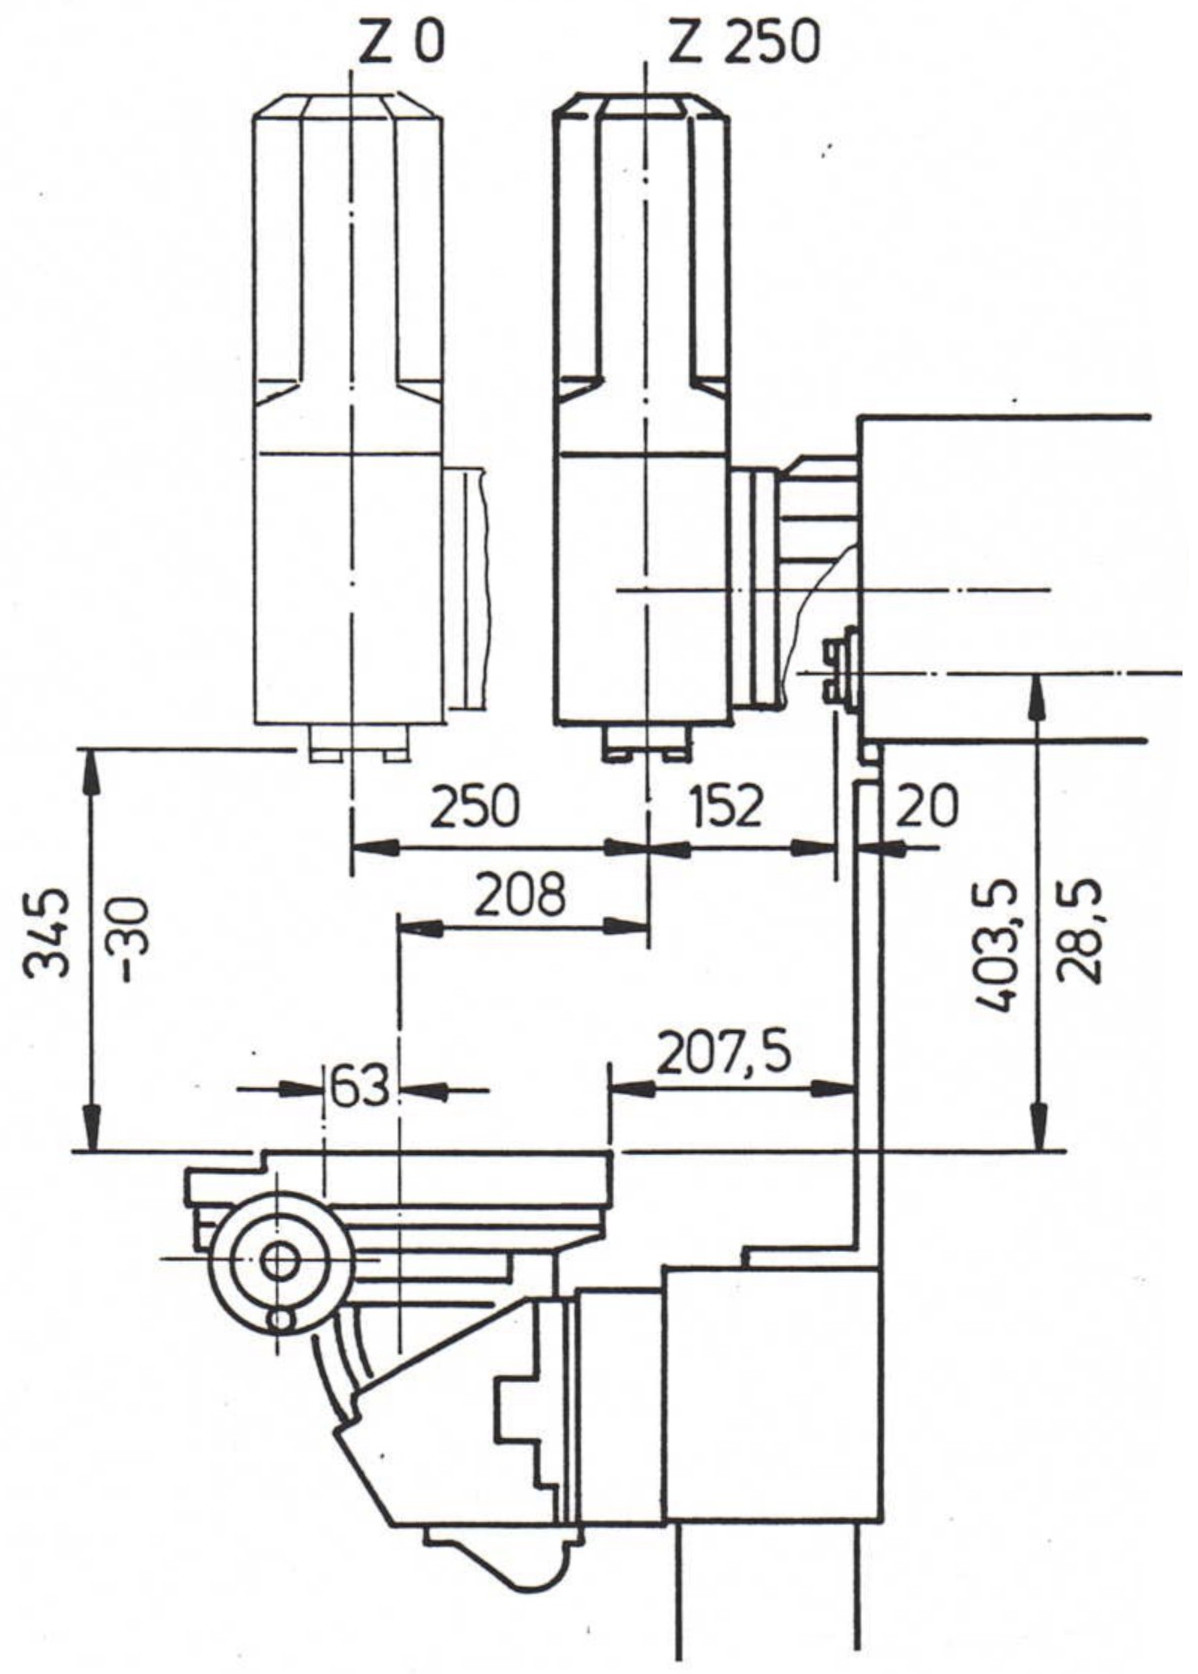
\includegraphics[width=0.75\textwidth]{chapter4/universal_rotary_table_dimensions.jpg}
\end{figure}

\section{Angle Adjustment Display for B-Axis - Universal Rotary Table}

For working with the ROD measurement system, it is necessary to convert the commonly used angular minutes and seconds from technical drawings into decimal values.

\subsection*{Conversion}
\[
\frac{\text{min.}}{60} + \frac{\text{sec.}}{3600} = 0,\dots^{\circ}
\]

The angle position is displayed on the \textbf{CNC 432 screen} with a resolution of $0.001^{\circ}$.

\subsection*{Examples}
\begin{itemize}
    \item \textbf{Example 1:} $18^{\circ} 36' 24'' = 18.606^{\circ}$
    \item \textbf{Example 2:} $63^{\circ} 06' 49'' = 63.113^{\circ}$
    \item \textbf{Example 3:} $203^{\circ} 58' 03'' = 203.967^{\circ}$
\end{itemize}

A fixed reference point in the ROD measuring system enables precise alignment of the workpiece and the restoration of the workpiece reference point after an interruption.

Before starting work, the reference point’s position should be determined based on the T-slots aligned parallel to the X-axis or Z-axis and noted separately.\footnotemark

\subsection*{Procedure}
\begin{itemize}
    \item Set the machine constant \textbf{C 75} to \textbf{0}, making the reference point and zero point identical.
    \item Move to reference points X, Y, Z. Move the rotary table with the hand crank until the display \textbf{B-RP} disappears. The text \textbf{READ-OUT} remains displayed.
    \item Rotate the table to the desired position. Ideally, the T-slots should be parallel to the X-movement.
    \item Enter the displayed \textbf{B} value on the screen into constant \textbf{C 75} with reversed signs (positive becomes negative and vice versa). This shifts the NP (new position) by the entered C 75 value from the RP (reference point).
    \item Move back to reference points X, Y, Z and drive the rotary table with the hand crank to \textbf{0}.
    \item After a power failure, only reference points X, Y, and Z need to be re-referenced. If B was also active, it must be referenced first, otherwise, X, Y, and Z will not be released.
\end{itemize}

\footnotetext{See the separate operating instructions for CNC 432 graphics.}
